\documentclass[10pt]{beamer} %
\usetheme{Boadilla}
\usecolortheme{beaver}
\usepackage[spanish]{babel}
\usepackage[utf8x]{inputenc}
\usefonttheme{professionalfonts}
\usepackage{times}
\usepackage{tikz}
\usepackage{amsmath}
\usepackage{tabulary}
\usepackage{pgfgantt}
\usepackage{verbatim}
\usetikzlibrary{arrows,shapes}
\usepackage{adjustbox}
\usepackage{soul}
\usepackage{listings}
\usepackage{adjustbox}
\newtheorem{Teo}{Teorema}
\setbeamertemplate{itemize item}{\color{red}$\blacksquare$}
\usepackage{hyperref}
\title{avance1}

\title{Hierarchical Bayesian Model for Insurance Claims}
%\institute[Yachay Tech]{School of Mathematical and Computational Sciences, Yachay Tech University, Ecuador}
\author[]{Erika Rivadeneira\\ School of Mathematical and Computational Sciences, Yachay Tech University, Ecuador
\vspace{0.25cm}
\\{\small{\textbf{Tutor:} Saba Rafael Infante\\School of Mathematical and Computational Sciences, Yachay Tech University, Ecuador\\\textbf{Cotutor:} Aracelis Hernández\\Department of Mathematics, Faculty of Science and Technology, University of Carabobo, Venezuela}}}




\date{\today}

\begin{document}
\tikzstyle{every picture}+=[remember picture]
\lstset{}   
\everymath{\displaystyle}

\begin{frame}
	\titlepage
\end{frame}

\begin{frame}
\frametitle{Summary}
\tableofcontents
\end{frame}

%------------------------------------------------------
\section{Introduction}
%------------------------------------------------------

\begin{frame}
\frametitle[9pt]{Introduction}
\begin{itemize}
    \item Insurance companies estimate the risk models to predict the magnitude of the claims and thus be able to determine the premiums that must be paid to the insured

    \item Pricing actuaries must use past information to develop probabilistic models that allow them to model the most important uncertainties involved in the process of losses. 
    \item Insurers must establish a statistical control model that allows for the reduction of unnecessary expenses
    \item Bayesian statistics allows us to include the experience of the experts through the preliminary information that is reflected in the choice of the a priori distributions that each of the parameters will have.
    
\end{itemize}

\end{frame}
%------------------------------------------------------------------------------------
\begin{frame}
\begin{itemize}
    \item In this sense, the purpose is to develop a methodology, under the Bayesian paradigm, allowing predictions to be made of the total future amounts of claims in order to determine the rate of premiums using a Bayesian hierarchical structure.
    \item The people insured in different age groups have different patterns in the frequency and severity of the reported claims
    \item It is introduced an additional category with the idea of being able to describe the regions of residence of the insured. 
    \item This spatial factor comes to represent the combined random effect of many elements on the severity and frequency of claims. 
\end{itemize}
\end{frame}

%---------------------------------------------------------------------------------------------

\section{Objectives}
%--------------------------------------------------------------
\begin{frame}{Objectives}
\begin{itemize}
    \item \textbf{General Objective}\\
    To predict the total number of claims using a hierarchical Bayesian model as a risk measure for insurance companies and to calculate the value of premiums under different principles.\\
    \item\textbf{Specific Objectives}
    \begin{itemize}
        \item Categorize the insured population by age classes in a specific unit of time. Add a spatial factor corresponding to the region of residence that represents the combined random effects of elements that influence the characterization of the claims.
	\item Implement a Markov Chain Monte Carlo (MCMC) algorithm that allows for the estimation of each of the parameters of the proposed model using a priori knowledge.
    \end{itemize}
\end{itemize}
\end{frame}
%--------------------------------------------------------------
\section{Methodology}
%--------------------------------------------------------------
\begin{frame}{Methodology}
\begin{itemize}
\item \textbf{Hierarchical Collective Risk Model}\\
\begin{itemize}
    \item The collective compound risk model is given by $$X_{t,i,a}=\sum_{j=1}^{N_{t,i,a}}Z_{t,i,a,j}$$ with $i=1,..,,I$, $t=1,...,T$ and $a=1,...,A$, in the time interval $(t-1,t)$.
    \item Where $Z_{t,i,a,j}$ is the amount of the $j-$th claim that occurred within the time interval $(t,t-1)$ for an age class $a$ in a region $i$.\\
        \begin{equation}\label{gamma1}
        Z_{t,i,a}\sim Gamma(\kappa_a,\theta_a)\quad with\quad \kappa_a>0,\theta_a>0
    \end{equation}
    and 
    \begin{equation}
    \label{poisson1}
    N_{t,i,a}\sim Poiss(M_{t,i,a}\lambda_a)\quad \lambda_a>0
    \end{equation} 
\end{itemize}
       
where 
\begin{itemize}
    \item $Z_{t,i,a}$ is the individual amount of the claim
    \item $M_{t,i,a}$ is the number of people insured in a time $t$ for an age class $a$ in the region $i$
    \item $\lambda_a$ is the average number of claims per individual per unit of time.
    \item $M_{t,i,a}$ implies a constant population in the time interval $(t-1,t)$ since the growth of the population is not modeled in this model.
\end{itemize}
    \end{itemize}
\end{frame}
%--------------------------------------------------------------
\begin{frame}
    Since the sum of these Gamma is also a Gamma, we have that 
    $$X_{t,i,a}|\theta_a,\kappa_a,n_{t,i,a}\sim Gamma(n_{t,i,a}\kappa_a,\theta_a)\quad with\quad \theta_a>0,\kappa_a>a$$
    Let's note that in (\ref{gamma1}) we see that the individual claim $Z_{t,i,a}\sim Gamm(\kappa_a,\theta_a)$ is the only variable that depends on age in this model.\\
    On the other hand, given that for a certain age class $a$ and region $i$ the insured population $M_ {t, i, a}$ varies over time, then the total number of claims $$\left\{X_{t, i, a},\quad t = 1, ..., T,\quad i = 1, ..., I,\quad a = 1, ..., A\right\}$$ are not identically distributed.
\end{frame}
\begin{frame}
\begin{itemize}
    \item \textbf{Spatial Effect}\\
    it is assumed that the insured population follows a normal distribution $$M_{t,i,a}\sim N(\mu_{t,i,a},\tau^{-1})\quad con \quad \tau>0$$ with precision $\tau$ and average 
\begin{equation}
	\label{mu_t,i,a}
	\mu_{t,i,a}=\beta_{a_0}+L_i+\beta_{1}e^{t\beta_{a_2}}
\end{equation}
 where $L_i$ represents the spatial factor for the region $i$ and $\beta_{a_0},\beta_{a_2}$ are parameters related to age. It's important to mention that the age of the insured population is independent of the information related to the region. 
\end{itemize}
    
\end{frame}
%--------------------------------------------------------------
\begin{frame}{Priori Distributions}

\begin{enumerate}[a)]
	\item Distributions that describe the value of the claims, the number of claims and the insured population:
	\begin{align*}
	X_{t,i,a}\sim Gamm(n_{t,i,a}\kappa_{a},\theta_a),\quad \theta_a>0,\kappa_a>0,\\
	N_{t,i,a}\sim Poiss(M_{t,i,a}\lambda_a),\quad \lambda_a>0,\\
	M_{t,i,a}\sim N(\mu_{t,i,a},\tau^{-1}),
	\end{align*}
	where $$\mu_{t,i,a}=\beta_{a_0}+L_i+\beta_1e^{t\beta_{a_2}}$$
	
\end{enumerate}

\end{frame}
%--------------------------------------------------------------
\begin{frame}{Priori Distributions}
\begin{enumerate}[b)]
   \item Distributions that describe the age and the regions
	\begin{align*}
	\theta_{a}&\sim Gamm(\alpha_{\theta},\beta_{\theta}),\\
	\kappa_{a}&\sim Gamm(\alpha_{	\kappa},\beta_{	\kappa}),\\
	\lambda_{a}&\sim Gamm(\alpha_{\lambda},\beta_{\lambda}),\\
	\beta_{a_0}=\beta_0+\varepsilon_a^0,&\textrm{ with }\varepsilon_a^0\sim N(0,\tau_{\varepsilon_0}^{-1}),\\
	\beta_{a_2}=\beta_2+\varepsilon_a^2,& \textrm{ with }\varepsilon_a^2\sim N(0,\tau_{\varepsilon_2}^{-1}),\\
	L&\sim NMV(0,\tau^{-1}Q^{-1}),
	\end{align*}
	where 
	\begin{align*}
	Q_{gh}=\left\{\begin{matrix}
	1+|\eta|\cdot m_g, \quad &g=h\\
	-\eta, \quad &g\neq h,g,h=1,2,...,I\\
	0,\quad &\textrm{otherwise}
	\end{matrix}\right.
	\end{align*}
	    These distributions are independent with $\alpha_{\lambda},\beta_{\lambda},\alpha_{\theta},\beta_{\theta},\alpha_{	\kappa},\beta_{	\kappa}$ non-negative amounts.
\end{enumerate}
    
\end{frame}
%--------------------------------------------------------------
\begin{frame}{Priori Distributions}
\begin{enumerate}[c)]
\item Distributions of the a priori hyperparameters
	\begin{align*}
	\beta_0\sim N(\mu_0,\tau_0^{-1})\\
	\beta_1\sim N(\mu_1,\tau_1^{-1})\\
	\beta_2\sim N(\mu_2,\tau_2^{-1})\\
	f(\eta)=\frac{1}{(1+\eta)^2},\quad \eta>0
	\end{align*}
	and $\psi=(\tau,\sigma,\tau_{\varepsilon_0},\tau_{\varepsilon_2},\alpha_{\theta},\beta_{\theta},\alpha_{\lambda},\beta_{\lambda},\alpha_{	\kappa},\beta_{	\kappa})$ follow Gamma distributions with known parameters $$\Rightarrow \psi \sim Gamm(\alpha_\psi,\beta_\psi)$$ where $\mu_0,\mu_1,\mu_2,\tau_0,\tau_1,\tau_2,\alpha_\psi,\beta_\psi$ are known values.
 \end{enumerate}   
\end{frame}
%--------------------------------------------------------------
\begin{frame}{Posterior Distributions}
$$P(\theta_{a}|\Theta_{-\theta_{a}},D_{t})\propto Gamm(\alpha_{\theta}+\sum_{t=1}^{T}\sum_{i=1}^{I}n_{t,i,a},\sum_{t=1}^{T}\sum_{i=1}^{I}X_{t,i,a}+\beta_{\theta})\quad\textrm{for }a=1,...,A$$
$$P(\lambda_{a}|\Theta_{-\lambda_{a}},D_{t})\propto Gamm(\alpha_{\lambda}+\sum_{t=1}^{T}\sum_{i=1}^{I}n_{t,i,a},\sum_{t=1}^{T}\sum_{i=1}^{I}M_{t,i,a}+\beta_{\lambda})\quad\textrm{for }a=1,...,A$$
\begin{align*}P(\beta_{0}|\Theta_{-\beta_{0}},D_{t})\propto& N\left(\frac{\tau_0\mu_0+\tau\sum_{t=1}^{T}\sum_{i=1}^{I}\sum_{a=1}^{A}\left( M_{t,i,a}-\varepsilon_a^0-L_i-\beta_{1}e^{t\beta_{a_2}}\right)}{\tau TIA+\tau_0},\\ 
&(\tau TIA+\tau_0)^{-1} \right)\\
P(\beta_{1}|\Theta_{-\beta_{1}},D_{t})\propto& N\left(\frac{\tau_1\mu_1+\tau\sum_{t=1}^{T}\sum_{i=1}^{I}\sum_{a=1}^{A}(M_{t,i,a}-\beta_{0}-\varepsilon_a^0-L_i)e^{t(\beta_{2}+\varepsilon_a^2)}}{\tau_1+\tau\sum_{t=1}^{T}\sum_{i=1}^{I}\sum_{a=1}^{A}e^{2t\beta_{a_2}}}
\\&,\left(\tau_1+\tau\sum_{t=1}^{T}\sum_{i=1}^{I}\sum_{a=1}^{A}e^{2t(\beta_{2}+\varepsilon_a^2)} \right)^{-1}\right)    
\end{align*}

\end{frame}
%--------------------------------------------------------------
\begin{frame}{Posterior Distributions}
\begin{align*}
    &P(\varepsilon_a^0|\Theta_{-\varepsilon_a^0},D_{t})\propto N\left( \frac{\tau\sum_{t=1}^{T}\sum_{i=1}^{I}\left(M_{t,i,a}-\beta_{0}-L_i-\beta_{1}e^{t(\beta_{2}+\varepsilon_a^2)}\right)}{(\tau TI+\tau_{\varepsilon_0})},(\tau TI+\tau_{\varepsilon_0})^{-1} \right)\\
    &P(\beta_2|\Theta_{-\beta_{2}},D_t)\propto e^{-\frac{\tau_2}{2}(\beta_{2}^2-2\beta_{2}\mu_2)-\frac{\tau}{2}\sum_{t=1}^{T}\sum_{i=1}^{I}\sum_{a=1}^{A}\left(\beta_{1}e^{t(\beta_2+\varepsilon_a^2)}-(M_{t,i,a}-\beta_{a_0}-L_i)\right)^2}\\
    &P(\varepsilon_a^2|\Theta_{-\varepsilon_a^2},D_{t})\propto e^{-\frac{\tau_{\varepsilon_2}}{2}(\varepsilon_a^2)^2-\frac{\tau}{2}\sum_{t=1}^{T}\sum_{i=1}^{I}\left(\beta_{1}e^{t(\beta_{2}+\varepsilon_a^2)}-(M_{t,i,a}-\beta_{a_0}-L_i) \right)^2}\\ &\textrm{for }a=1,...,A\\
    &P(\tau|\Theta_{-\tau},D_{t})\propto Gamm\left(\frac{1}{2}TIA+\alpha_\tau, \frac{1}{2}\sum_{t=1}^{T}\sum_{i=1}^{I}\sum_{a=1}^{A}(M_{t,i,a}-\mu_{t,i,a})^2+\beta_\tau\right)\\
    &P(\tau_{\varepsilon_0}|\Theta_{-\tau_{\varepsilon_0}},D_{t})\propto Gamm\left(\frac{A}{2}+\alpha_{\tau_{\varepsilon_0}},\beta_{\tau_{\varepsilon_0}}+\frac{1}{2}\sum_{a=1}^{A}(\varepsilon_a^0)^2 \right)
\end{align*}
    
\end{frame}
%--------------------------------------------------------------
\begin{frame}{Posterior Distributions}
    \begin{align*}
        &P(\tau_{\varepsilon_2}u|\Theta_{-\tau_{\varepsilon_2}},D_{t})\propto Gamm\left(\frac{A}{2}+\alpha_{\tau_{\varepsilon_2}},\beta_{\tau_{\varepsilon_2}}+\frac{1}{2}\sum_{a=1}^{A}(\varepsilon_a^2)^2 \right)\\
        &P(\alpha_\theta|\Theta_{-\alpha_\theta},D_{t})\propto \Gamma(\alpha_{\theta})^{-A}\beta_{\theta}^{A\alpha_{\theta}}\alpha_{\theta}^{\alpha_{\alpha_{\theta}}-1}e^{-\beta_{\alpha_{\theta}}\alpha_{\theta}}\left(\prod_{a=1}^{A}\theta_{a}^{\alpha_{\theta}-1}\right)\\
        &P(\alpha_\lambda|\Theta_{-\alpha_\lambda},D_{t})\propto \Gamma(\alpha_{\lambda})^{-A}\beta_{\lambda}^{A\alpha_{\lambda}}\alpha_{\lambda}^{\alpha_{\alpha_{\lambda}}-1}e^{-\beta_{\alpha_{\lambda}}\alpha_{\lambda}}\left(\prod_{a=1}^{A}\lambda_{a}^{\alpha_{\lambda}-1}\right)\\
        &P(\beta_{\theta}|\Theta_{-\beta_{\theta}},D_{t})\propto Gamma\left(A\alpha_{\theta}+\alpha_{\beta_{\theta}},\beta_{\beta_{\theta}}+\sum_{a=1}^{A}\theta_{a} \right)\\
        &P(\beta_{\lambda}|\Theta_{-\beta_{\lambda}},D_{t})\propto Gamma\left(A\alpha_{\lambda}+\alpha_{\beta_{\lambda}},\beta_{\beta_{\lambda}}+\sum_{a=1}^{A}\lambda_{a} \right)\\
    \end{align*}
\end{frame}
%--------------------------------------------------------------
\begin{frame}{Posterior Distributions}
For the spatial variable, we have to study $ mg $ neighboring regions, then the variance-covariance matrix of the multivariate normal distribution is given by
\begin{align*}
	\sigma^{-1}\cdot\left( \begin{array}{cc}
	1+|\eta|\cdot mg & -\eta \\
	-\eta & 1+|\eta|\cdot mg
	\end{array} \right)^{-1} =\left( \begin{array}{cc}
	P&S\\
	S&P
	\end{array}\right)
\end{align*}
whence, the correlation coefficient is given by 
$$\rho =\frac{\eta}{1+\eta}$$
So that,
\begin{align*}
&P(L_i|\Theta_{-L_i},D_{t})\propto\left[\prod_{t=1}^{T}\prod_{a=1}^{A}e^{-\frac{\tau}{2}(M_{t,i,a}-\mu_{t,i,a})^2}\right]\cdot e^{-\frac{1}{2P^2(1-\rho^2)\left(L_1^2+L_2^2-2\rho L_1L_2\right)}}\\
    &P(\eta|\Theta_{\eta},D_{t})\propto \frac{1}{(1+\eta)^2P\sqrt{1-\rho^2}}e^{-\frac{1}{2P^2(1-\rho^2)}(L_1^2+L_2^2-2\rho L_1L_2)}\\
    &P(\sigma|\Theta_{-\sigma},D_{t})\propto \frac{1}{P^2}\sigma^{\alpha_\sigma-1}e^{-\sigma \beta_\sigma}e^{-\frac{1}{2P^2(1-\rho^2)}(L_1^2+L_2^2-2\rho L_1L_2)}
\end{align*}

\end{frame}
%--------------------------------------------------------------
\section{Simulation Studies and Model Fitting}
\begin{frame}{Model Fitting}
    It is assumed that: \\
\begin{itemize}
	\item \textbf{Claim Frecuency Parameters}
	\begin{itemize}
		\item $\lambda_{a}\sim Gamma(40,200)$ for any $a=1,2,...,7$
	\end{itemize}
	\item \textbf{Claim Severity Parameters}
	\begin{itemize}
		\item $\kappa_{a}=1$ for any $a=1,2,...,7$
		\item $\theta_{a}\sim Gamma(400,10000)$ for any $a=1,2,...,7$ 
	\end{itemize}
	\item \textbf{Population Parameters}
\begin{align*}
    \beta_0&\sim N(20, 10^4)\\
    \beta_1&\sim N(30, 10^4)\\
    \beta_2&\sim N(0.015, 10^2)
\end{align*}
\item For all other hyperparameters, the priors which contain little information are presented as follows:
\begin{align*}
    \tau,\alpha_\lambda,\beta_\lambda,\alpha_\theta,\beta_\theta&\sim Gamma(0.001,0.001),\\
    \tau_{\varepsilon_0}&\sim Gamma(1,10000),\\
    \tau_{\varepsilon_2}&\sim Gamma(1,100),\\
    \sigma&\sim Gamma(1,0.005),\\
    \eta&\sim Pareto(1,1).
\end{align*}
\end{itemize}

\end{frame}
%--------------------------------------------------------------

\begin{frame}{Results}
\begin{figure}
    \centering
    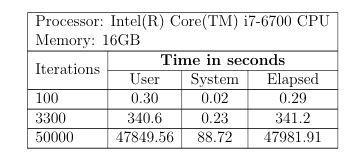
\includegraphics[width=0.75\textwidth]{Tab1.png}
    \caption{Compilation time of Gibbs sampler algorithm}
    \label{fig:TAB1}
\end{figure}
\end{frame}

\begin{frame}{Results}
    \begin{figure}[h]
    \centering
    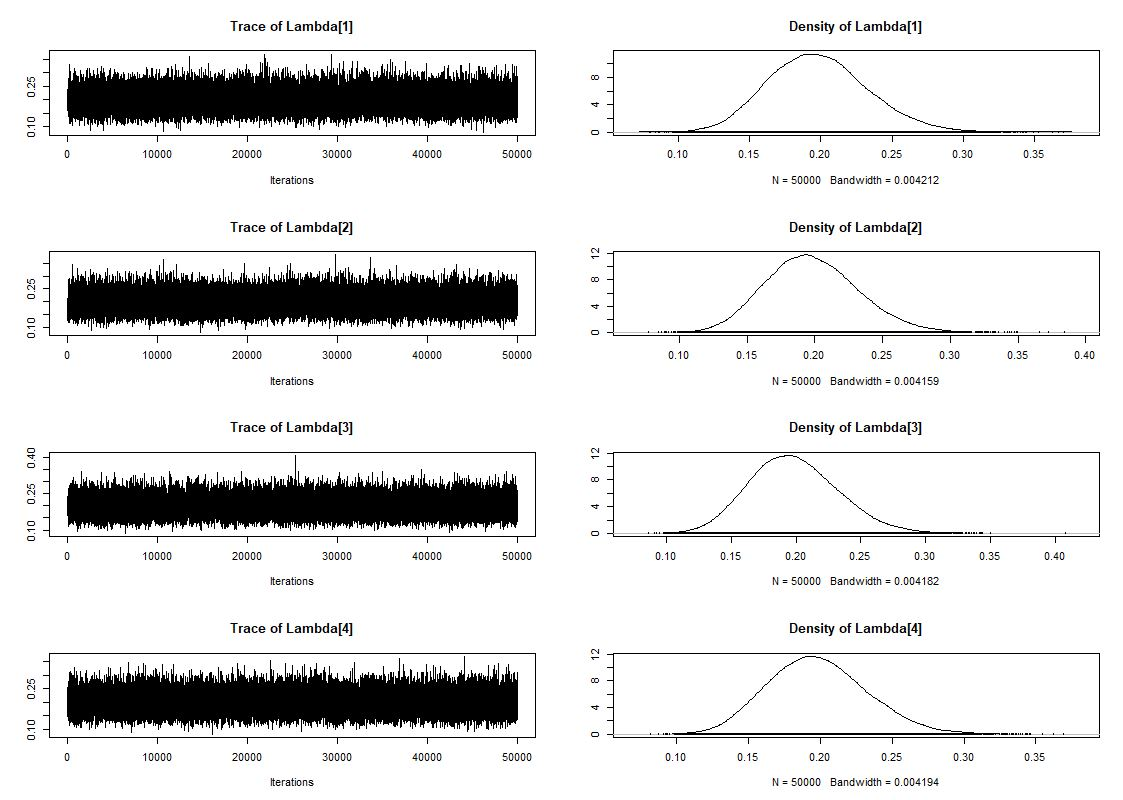
\includegraphics[width=0.8\textwidth]{Lambda1.JPG}
    \caption{Trace plot and the posterior distribution of $\lambda$ for $a=1,2,3,4$}
    \label{Lambda}
\end{figure}
\end{frame}

\begin{frame}{Results}
    \begin{figure}[H]
    \centering
    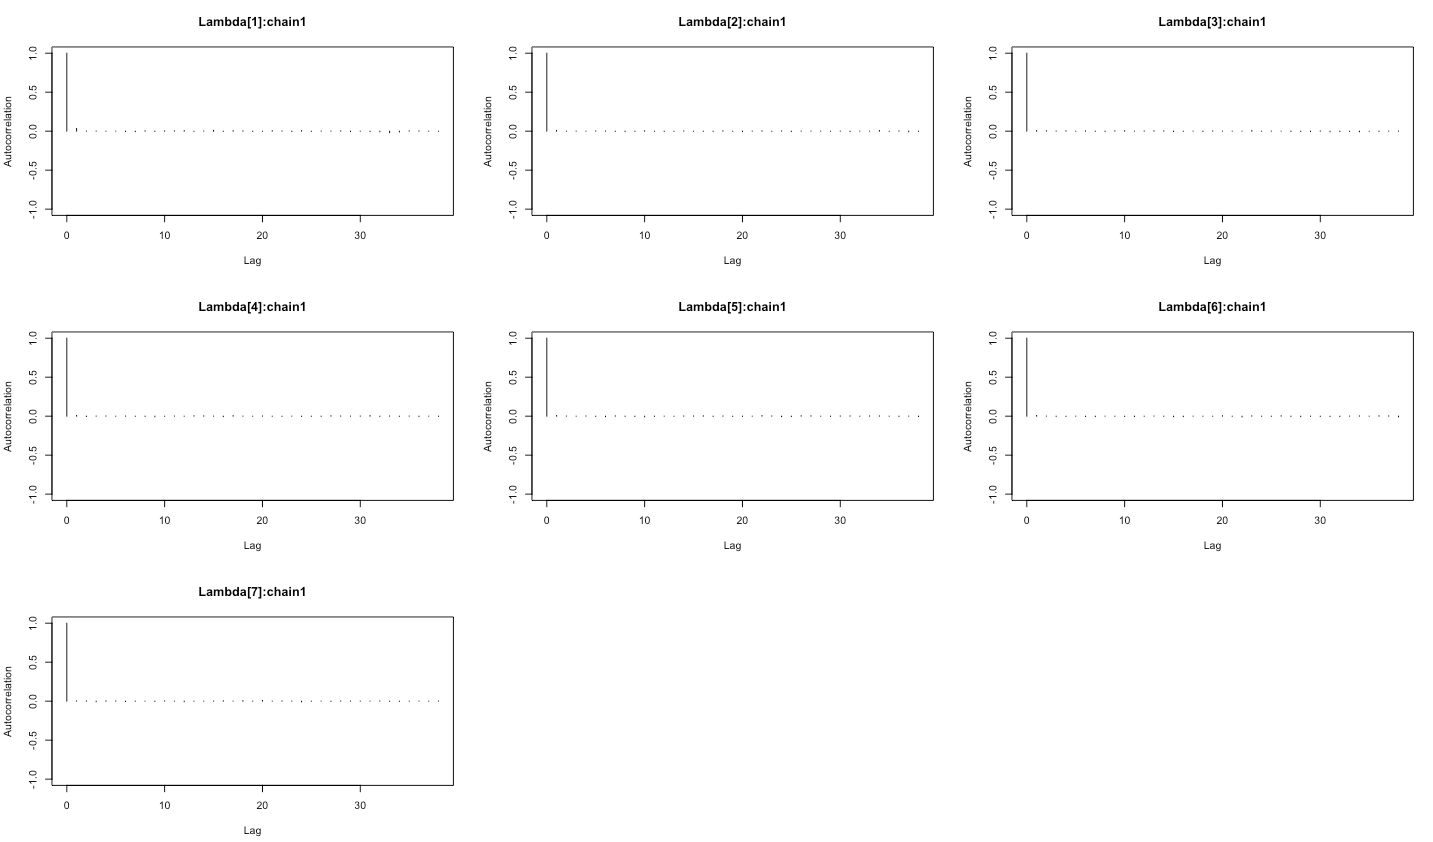
\includegraphics[width=1\textwidth ]{Auto_cor_LAMBDA.png}
    \caption{Autocorrelation of $\lambda$, for $a=1,..,7$}
    \label{autocorLambda}
\end{figure}
\end{frame}

\begin{frame}{Results}
    \begin{figure}[H]
    \centering
    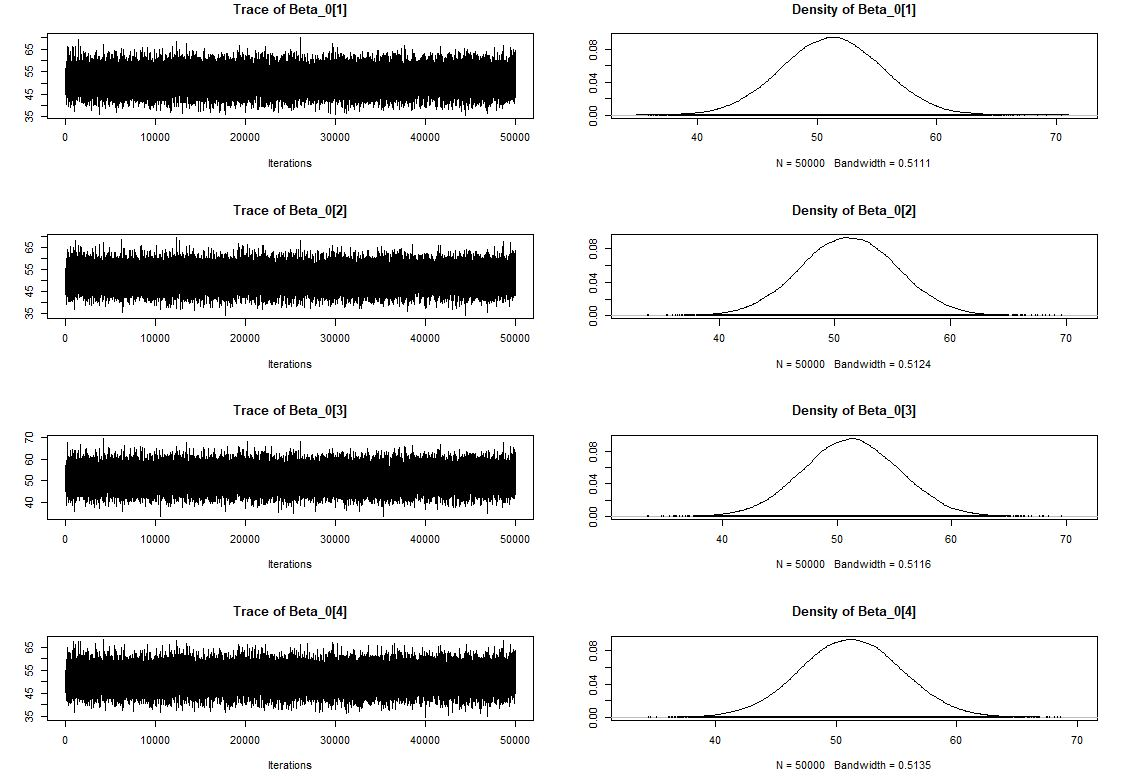
\includegraphics[width=0.8\textwidth]{Beta_a01.JPG}
    \caption{Trace plot and the posterior distribution of $\beta_0$ for $a=1,2,3,4$}
    \label{betaa0}
\end{figure}
\end{frame}

\begin{frame}{Results}
    \begin{figure}[H]
    \centering
    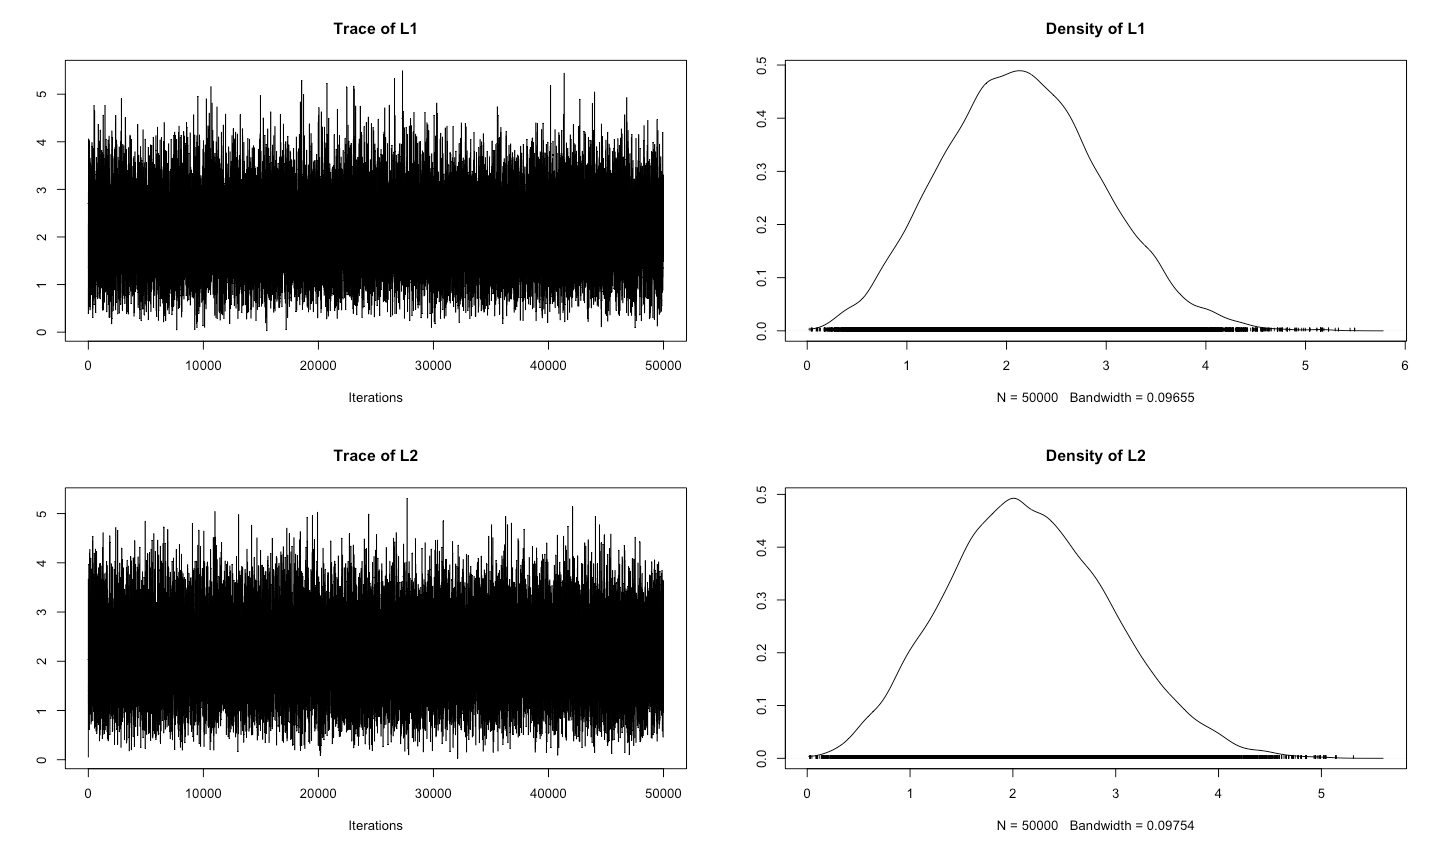
\includegraphics[width=0.4\textwidth ]{L_trace.png}
    \caption{Trace plot and the posterior distribution of $L_i$ for $i=1,2$}
    \label{L_i}
\end{figure}

\begin{figure}[H]
    \centering
    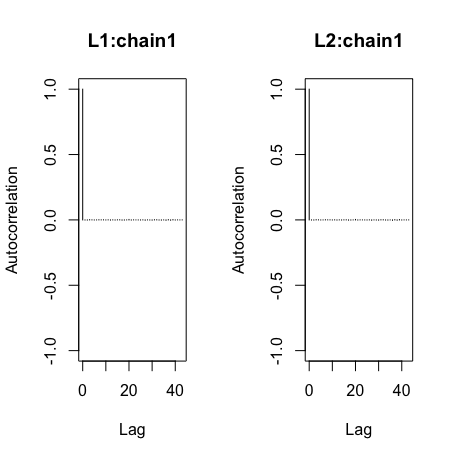
\includegraphics[width=0.27\textwidth ]{Auto_cor_L.png}
    \caption{Autocorrelation of $L_i$ for $i=1,2$}
    \label{autocorL}
\end{figure}
\end{frame}

\begin{frame}{Summary}
    \begin{figure}
        \centering
        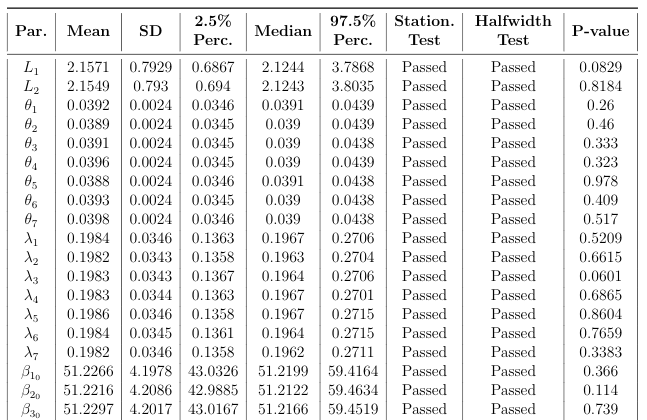
\includegraphics[width=0.8\textwidth ]{summary1.png}
        \caption{Statistical summary of some parameters}
        \label{fig:summary}
    \end{figure}
\end{frame}

\section{Predictions and Premium Determination}
\begin{frame}{Predictions}
    \begin{figure}[H]
    \centering
    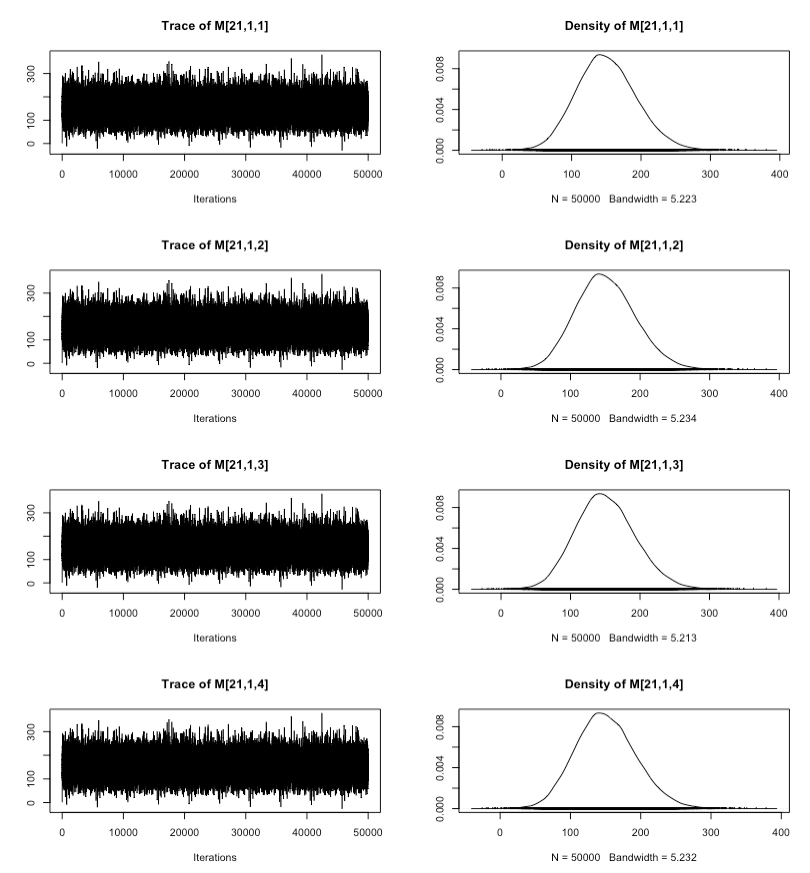
\includegraphics[width=0.5\textwidth ]{M21_1.png}
    \caption{Prediction of Insured Population for $21st$ Time Unit - Region $1$ - Age classes $1,2, 3$ and $4$}
    \label{predictionM1}
\end{figure}
\end{frame}

\begin{frame}{Predictions}
    \begin{figure}[H]
    \centering
    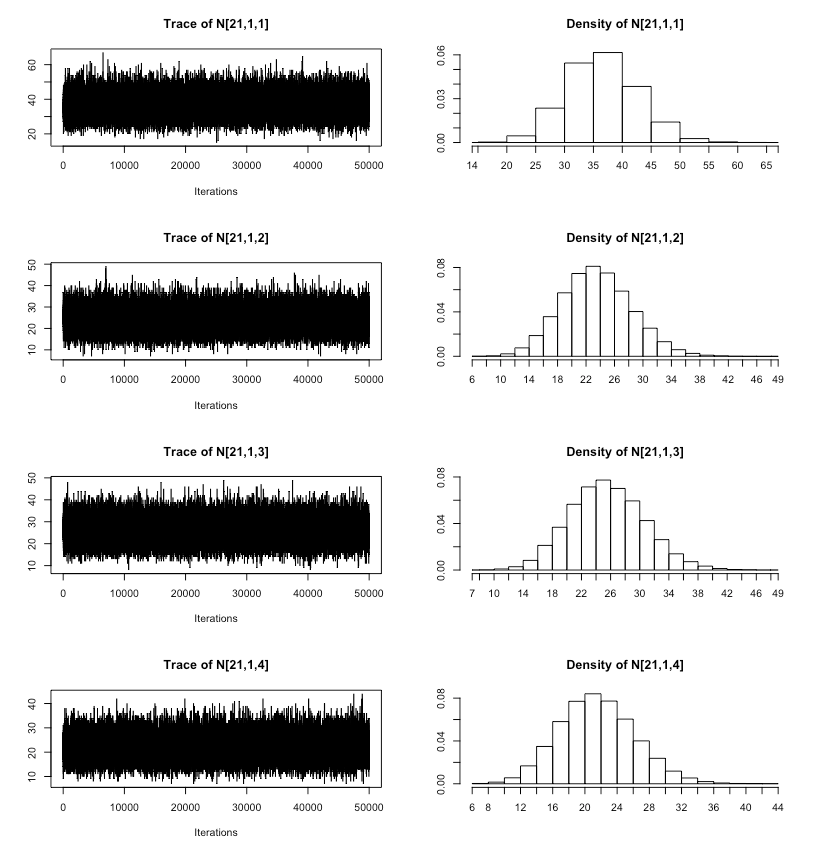
\includegraphics[width=0.5\textwidth ]{N21_1.png}
    \caption{Prediction of Number of Claims for $21st$ Time Unit - Region $1$ - Age classes $1,2, 3$ and $4$}
    \label{predictionN1}
\end{figure}
\end{frame}

\begin{frame}{Predictions}
    \begin{figure}[H]
    \centering
    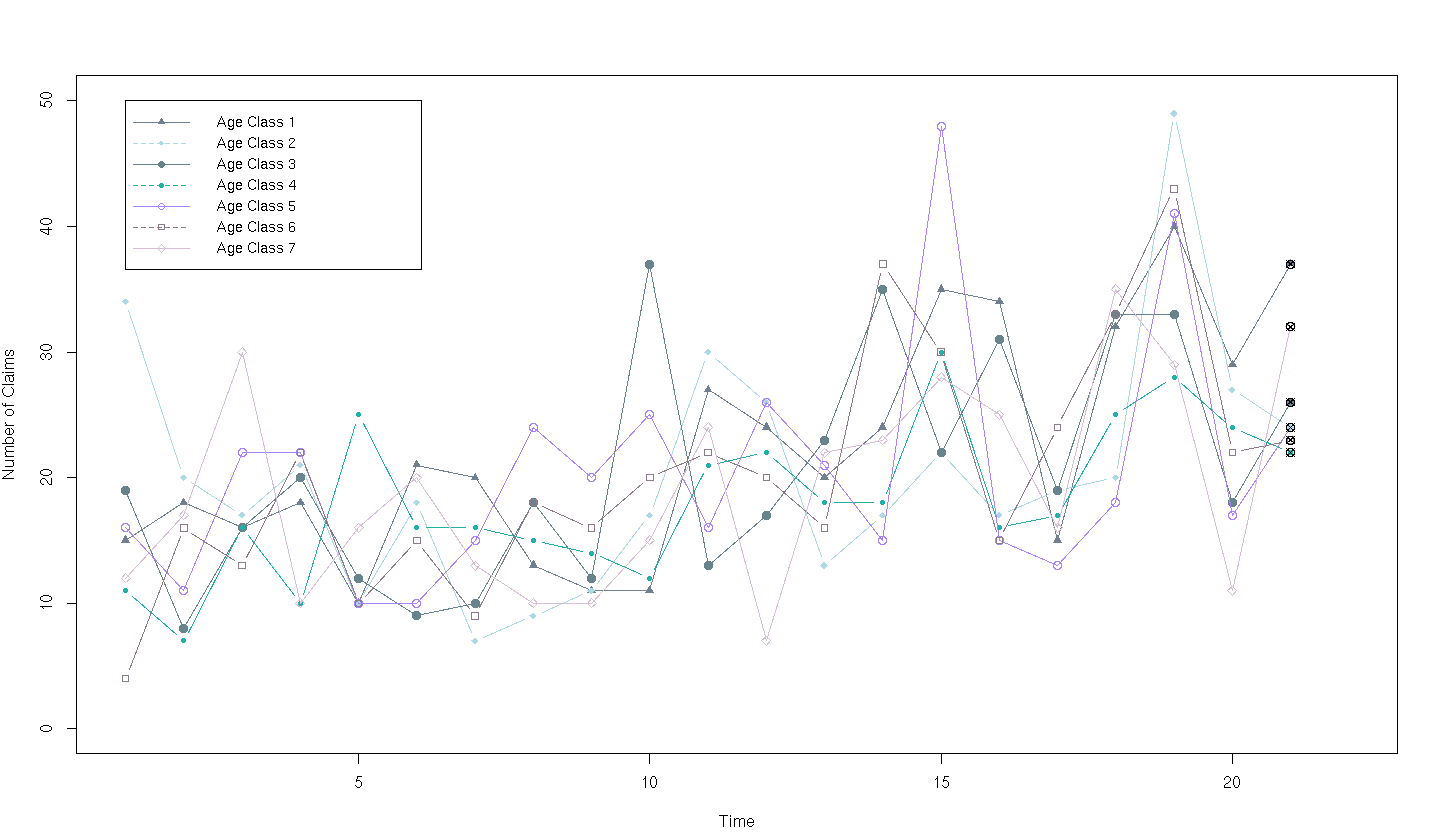
\includegraphics[width=0.7\textwidth ]{N_pred_REGION1.png}
    \caption{Claim Number with Prediction for all Age Classes - Region 1 }
    \label{predictionN_REGION1}
\end{figure}
\end{frame}

\begin{frame}{Predictions}
    \begin{figure}[H]
    \centering
    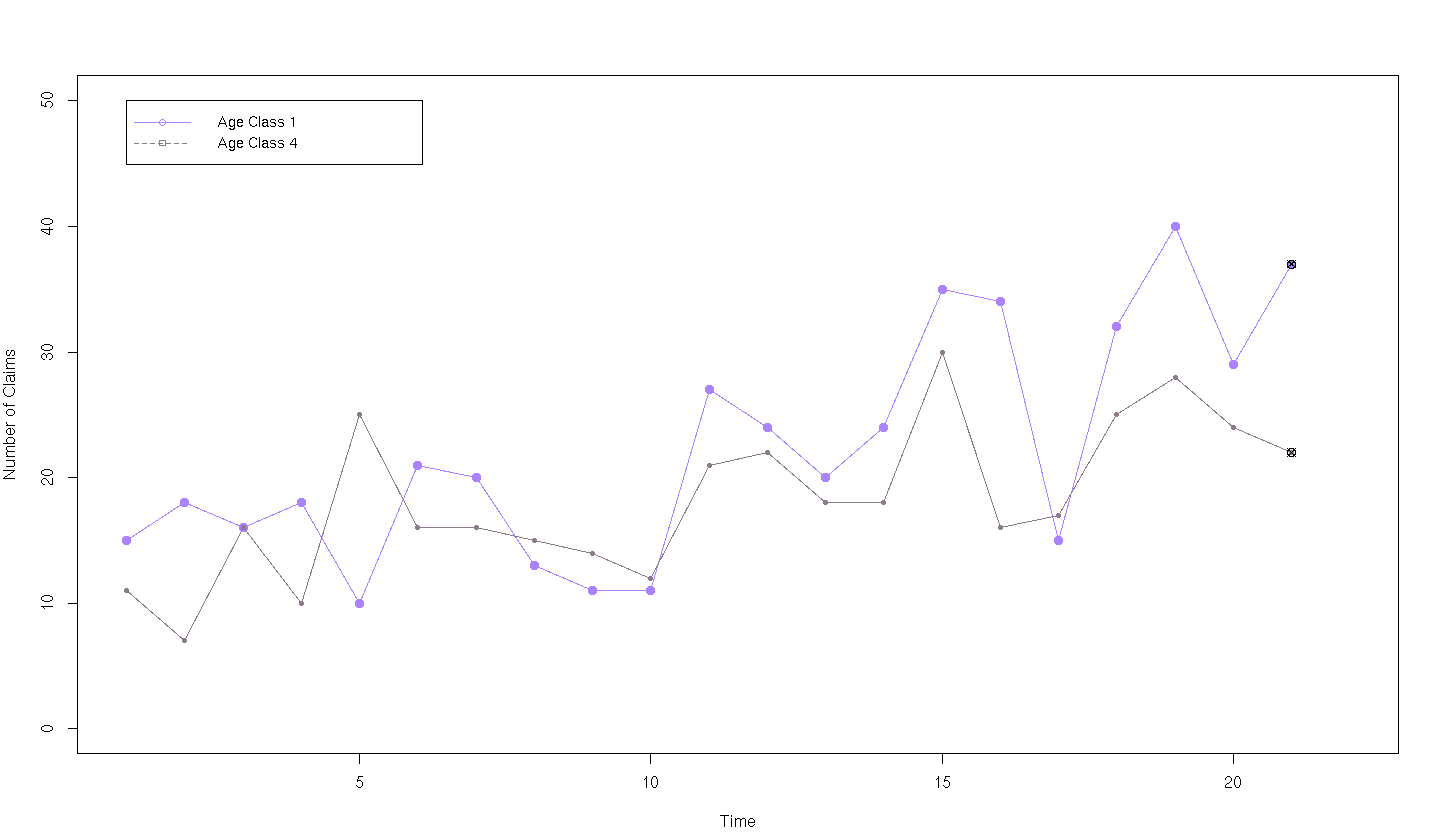
\includegraphics[width=0.5\textwidth ]{N_pred_AGE1&4_REGION1.png}
    \caption{Claim Number with Prediction for Region 1 - Age Groups 1 and 4 }
    \label{predictionN_AGE1and4}
\end{figure}
\end{frame}

\begin{frame}{Predictions}
   \begin{figure}[H]
    \centering
    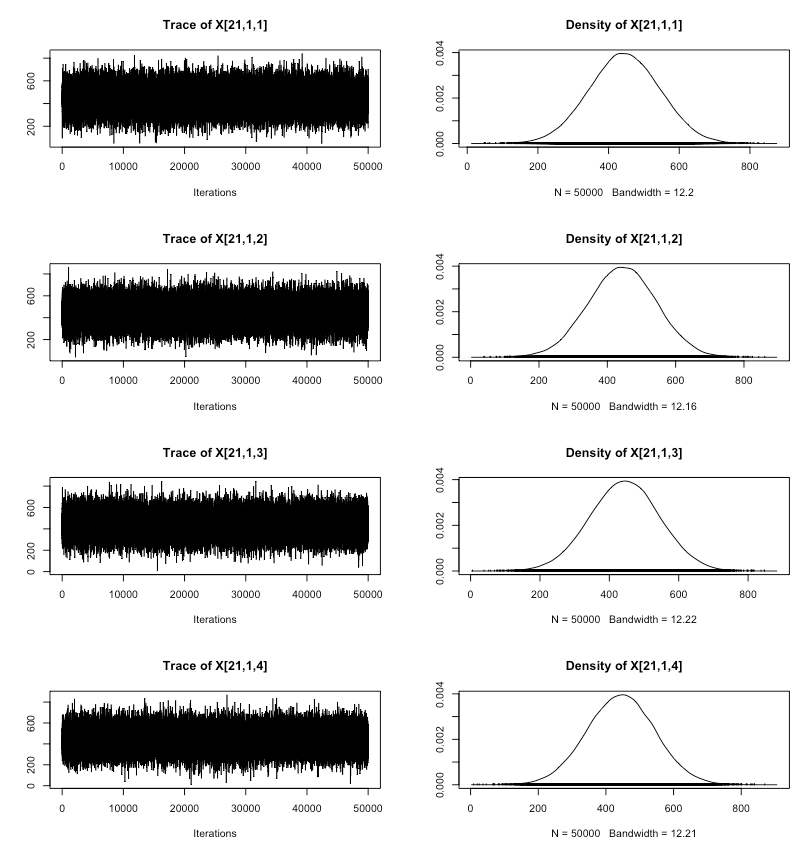
\includegraphics[width=0.5\textwidth ]{X_21_1.png}
    \caption{Prediction of Total Claim Amount for $21st$ Time Unit - Region $1$ - Age classes $1,2, 3$ and $4$}
    \label{predictionX1}
\end{figure} 
\end{frame}

\begin{frame}{Predictions}
   \begin{figure}[H]
    \centering
    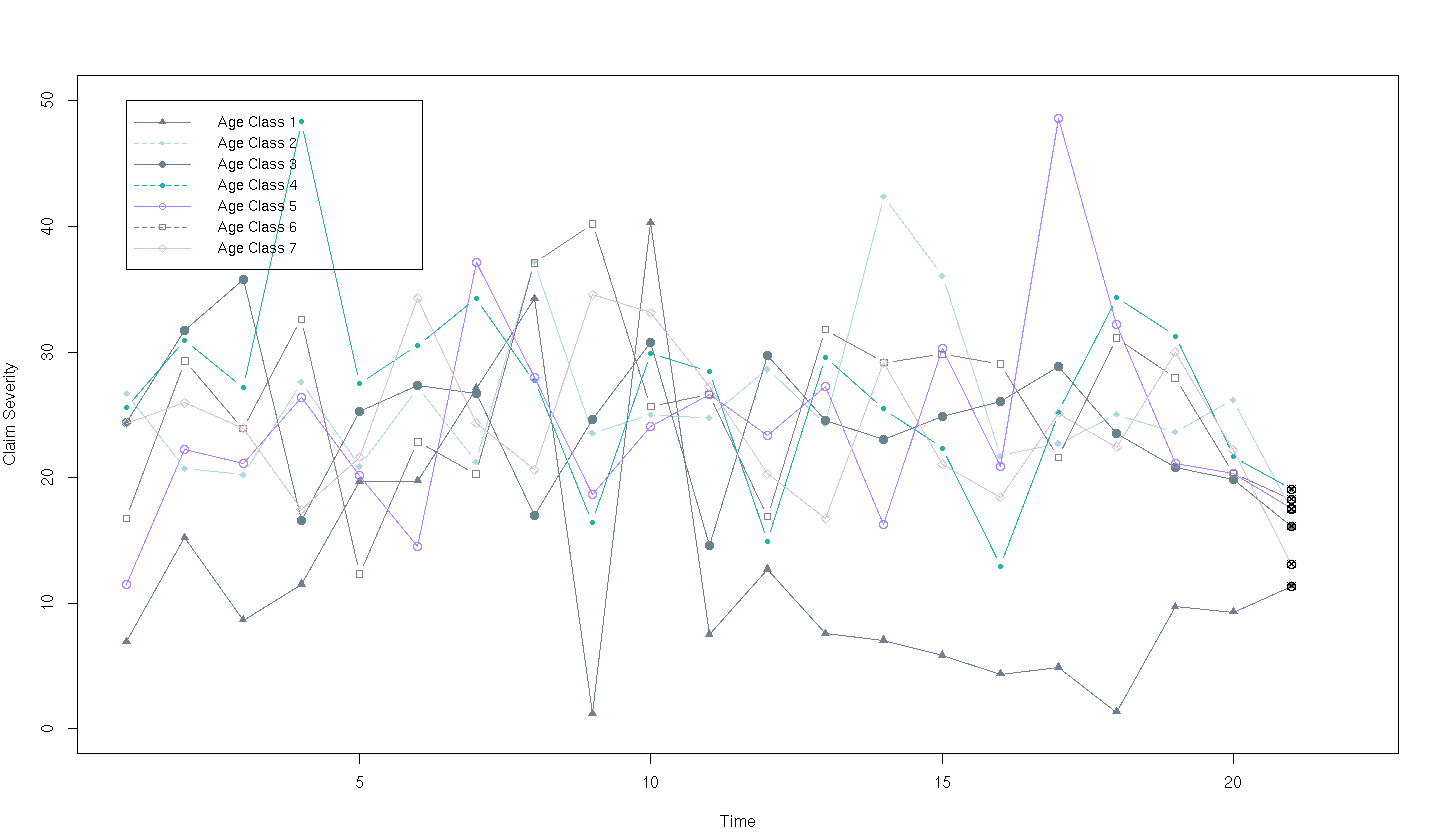
\includegraphics[width=0.7\textwidth ]{Average_claim_amount_REGION1.png}
    \caption{Average Amount Per Claim with Prediction in Region 2 - All Age Groups  }
    \label{predictionX_average_region2}
\end{figure} 
\end{frame}
\begin{frame}{Statistical Predictions Summary}
    \begin{figure}
        \centering
        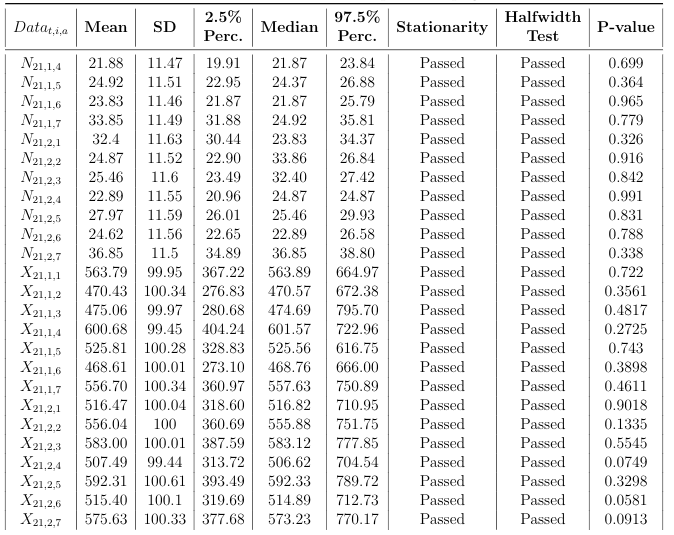
\includegraphics[width=0.7\textwidth]{summary2.png}
        \caption{Statistical Prediction Summary of Claim Number and Total Claim Amount for $21st$ Time Unit}
        \label{fig:my_label}
    \end{figure}
\end{frame}


\begin{frame}{Premiums Determination}
    \begin{figure}
        \centering
        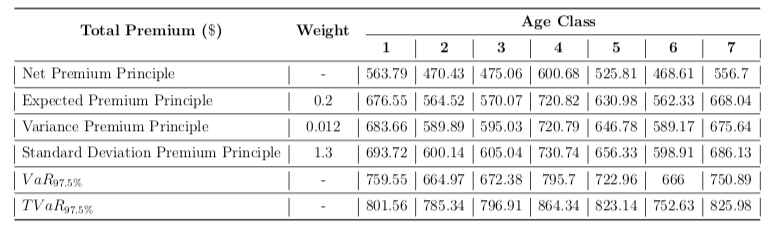
\includegraphics[width=1\textwidth]{Premiums.png}
        \caption{Total Premiums for $21^{st}$ Time Unit in Region 1 Using Predicted Results}
        \label{fig:my_label}
    \end{figure}
\end{frame}

\begin{frame}{Premiums Determination}
    \begin{figure}
        \centering
        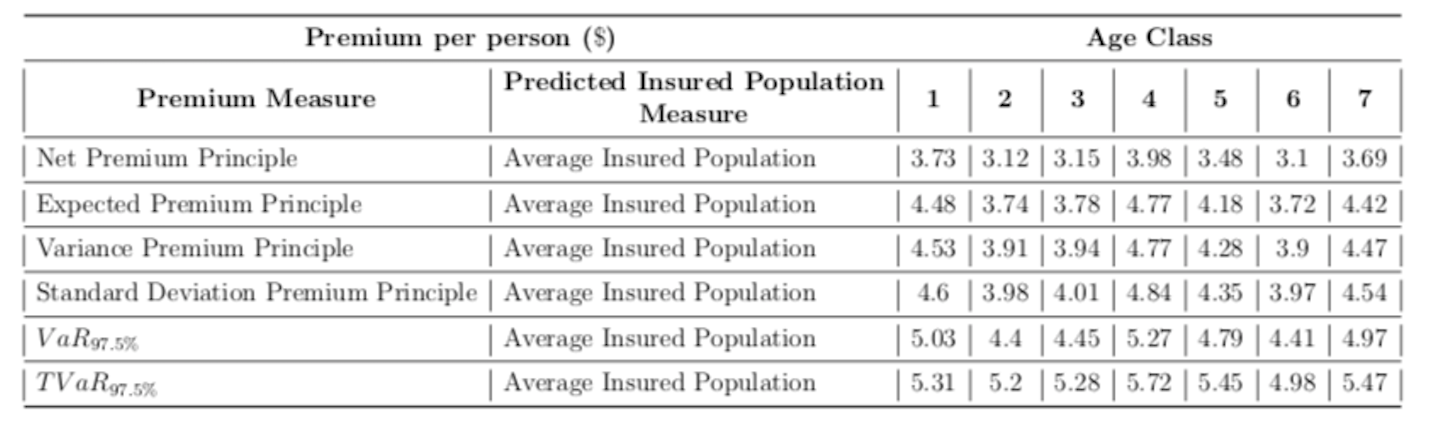
\includegraphics[width=1\textwidth]{PolicyHolder.png}
        \caption{Premium Per Policyholder for $21^{st}$ Time Unit in Region 1}
        \label{fig:my_label}
    \end{figure}
\end{frame}
\section{Conclusions}
\begin{frame}{Conclusions}
    \begin{itemize}
        \item It is possible to achieve a prediction of the total amount of claims under a Bayesian hierarchical framework. 
        \item The prediction of future claims plays an important role in the measurement of risk for health insurance providers therefore it is a primary issue. 
        \item Different patterns are presented in the frequency and severity of the claim reported in different age classes of the insured. 
        \item The proposed model introduces one more category, the spatial factor independent of the existing age classification, to describe the regions of the insured's residence. 
     \item The traces in all studies show signs of convergence.
     \item Predictions are made for the unit of time 21, which includes the insured population, the number of claims and the amounts of the claims after generating the values of true parameters.
     \item Premiums can be calculated under various premium principles, depending on the expected claim amounts.
    \end{itemize}
\end{frame}

\begin{frame}
\centering
    \textbf{Thank you all!}
\end{frame}

\end{document}